\documentclass{article}
\usepackage{amsmath}
\usepackage{cancel}
\usepackage{xcolor}
\usepackage{tikz}


% Set page size and margins
% Replace `letterpaper' with `a4paper' for UK/EU standard size
\usepackage[letterpaper,top=2cm,bottom=2cm,left=3cm,right=3cm,marginparwidth=1.75cm]{geometry}


\usepackage[colorlinks=true, allcolors=blue]{hyperref}



% Language setting
% Replace `english' with e.g. `spanish' to change the document language
\usepackage[english]{babel}

% Set page size and margins
% Replace `letterpaper' with `a4paper' for UK/EU standa rd size
\usepackage[letterpaper,top=2cm,bottom=2cm,left=3cm,right=3cm,marginparwidth=1.75cm]{geometry}

% Useful packages
\usepackage{amsmath}
\usepackage{amssymb}
\usepackage{graphicx}
\usepackage{qtree}
\usepackage{xcolor}

\title{Etude 8 - Four the Same}
\author{BobbyTables - Beckham Wilson, Kevin Albert, Dyrel Lumiwes, Raaid Taha}

\begin{document}
\maketitle

\begin{abstract} Imagine a square platform that can rotate about its centre. On each of the four corners
of the platform is an identical container with a lid. Inside each container is a coin.
Each coin can show either heads or tails. The coins are also identical. No part of the
apparatus can be marked not the coins, containers, or any part of the platform. \\

\begin{itemize}
    \item Initially, the containers with coins are locked and you cannot look inside.
    \item When you press ‘start’ the coins in the containers are shaken up, so that each one is randomly placed in a certain position, either heads or tails.
    \item When you press ‘continue’ the lights go out and the platform turns around its centre and stops at a random point (like a roulette wheel). The lights come on again.
    \item The containers unlock and you are now allowed to look inside any two containers (as soon as you have opened two the others lock again).
    \item You may change the way the two coins you can see are placed, from heads to tails or vice versa (you may change none, one, or two).
    \item You close the containers and press ‘continue’; the previous three steps are repeated until you have solved the puzzle.
    \item The puzzle is solved when all the coins are turned the same way, either all heads or all tails. When this state has been reached a bell will ring to tell you that you have solved the puzzle successfully.
\end{itemize}
\end{abstract}

\section{Introduction}

After much deliberation, anguish and trial and error, we have devised a solution that will solve this puzzle in 5 steps.


\section{Thought Process}

\subsection{Examining the problem}

Firstly let us examine the problem. The four non-winning states for which we will be able to start without instantly winning in zero steps are the following:\\



\begin{figure}[h]
    \centering
    \begin{minipage}[t]{0.2\textwidth}
        $\begin{bmatrix}
        H & T \\
        H & T 
        \end{bmatrix}$
        \caption{}
    \end{minipage}
    \begin{minipage}[t]{0.2\textwidth}
       $\begin{bmatrix}
        H & T \\
        T & H 
        \end{bmatrix}$
        \caption{}
    \end{minipage}
    \begin{minipage}[t]{0.2\textwidth}
        $\begin{bmatrix}
        T & H \\
        T & T 
        \end{bmatrix}$
        \caption{}
    \end{minipage}
     \begin{minipage}[t]{0.2\textwidth}
        $\begin{bmatrix}
        H & T \\
        H & H 
        \end{bmatrix}$
        \caption{}
    \end{minipage}
\end{figure}
Figure 1 is where two coins of the same face value are located adjacent to each other. Figure 2 is where the coins of the same face value are located along the diagonal of the state. Lastly, the final two figures are states which have three coins of the same face value and one coin of a different face value. We ignore the different orientations of each state because they don't affect the relative position of the coins. Below, we have noted all possible states for each figure. 
\\
\begin{center}
States of Figure 1
\end{center}
\begin{center}
$\begin{bmatrix}
        H & T \\
        H & T 
    \end{bmatrix}$
        = 
    $\begin{bmatrix}
        T & H \\
        T & H 
    \end{bmatrix}$
       =
    $\begin{bmatrix}
        H & H \\
        T & T 
    \end{bmatrix}$
        =
    $\begin{bmatrix}
        T & T \\
        H & H 
    \end{bmatrix}$
\end{center}
\begin{center}
States of Figure 2
\end{center}
\begin{center}
$\begin{bmatrix} 
        H & T \\
        T & H
        \end{bmatrix}$
        =
        $\begin{bmatrix}
        T & H \\
        H & T 
        \end{bmatrix}$
\end{center}
\begin{center}
States of Figure 3
\end{center}
\begin{center}
$\begin{bmatrix} 
        T & H \\
        T & T
        \end{bmatrix}$
        =
        $\begin{bmatrix}
        T & T \\
        T & H 
        \end{bmatrix}$
         =
        $\begin{bmatrix}
        T & T \\
        H & T 
        \end{bmatrix}$
         =
        $\begin{bmatrix}
        H & T \\
        T & T 
        \end{bmatrix}$
\end{center}
\begin{center}
States of Figure 4
\end{center}
\begin{center} 
    $\begin{bmatrix}
        H & H \\
        T & H 
    \end{bmatrix}$
        =
    $\begin{bmatrix}
        H & H \\
        T & H 
    \end{bmatrix}$
        =
    $\begin{bmatrix}
        T & H \\
        H & H 
    \end{bmatrix}$
        =
    $\begin{bmatrix}
        T & H \\
        H & H 
    \end{bmatrix}$
\end{center}
Our thought process for deriving the solution was to end up with 
$\begin{bmatrix} 
        H & T \\
        T & H
        \end{bmatrix}$ state which we know no matter what diagonal is picked we will win. Hence we arrive at this state via $\begin{bmatrix}
        T & H \\
        H & H 
        \end{bmatrix}$ $\rightarrow$ $\begin{bmatrix} 

        T & H \\
        T & H 
        \end{bmatrix}$ $\rightarrow$  $\begin{bmatrix} 

        H & T \\
        T & H
        \end{bmatrix}$ 

\subsection*{Clarification of Strategy}

Upon reaching the $\begin{bmatrix} H & T \\
        T & H
        \end
        {bmatrix}$ it results in a win in one move. Flipping both coins on the diagonal
meaning the other diagonal coins now matches. Since all four coins are now the same (either heads or tails), the game is won.


\section{Solution}
Our solution requires at most 5 moves listed as 3.1 to 3.5 below.

\subsection{Check Diagonal}

\begin{center}
$\begin{bmatrix} 
    \colorbox{yellow}{?} & ? \\
    ? & \colorbox{yellow}{?}
\end{bmatrix}$ $\rightarrow$ $\begin{bmatrix}
    H & ? \\
    ? & H 
\end{bmatrix}$, Regardless of what you see, make both coins heads.
\end{center}

If we didn't win immediately then the remaining states after step 1 are: 
$\begin{bmatrix}
    H & H \\
    T & H 
\end{bmatrix}$ or $\begin{bmatrix}
    H & T \\
    T & H 
\end{bmatrix}$.

\subsection{Check Adjacent}

\begin{center}
$\begin{bmatrix} 
    \colorbox{yellow}{?} & \colorbox{yellow}{?}  \\
    ? & ?
\end{bmatrix}$ $\rightarrow$ $\begin{bmatrix}
    H & H \\
    ? & ? 
\end{bmatrix}$, Regardless of what you see, make both coins heads.
\end{center}

If we didn't win immediately then the remaining state after step 2 is:
$\begin{bmatrix}
    T & H \\
    H & H 
\end{bmatrix}$.

\subsection{Check Diagonal}

\begin{center}
If $\begin{bmatrix}
    H & ? \\
    ? & H 
\end{bmatrix}$ $\rightarrow$ $\begin{bmatrix}
    H & ? \\
    ? & T 
\end{bmatrix}$, flip one of the H to T.
\end{center}

\begin{center}
If $\begin{bmatrix}
    T & ? \\
    ? & H 
\end{bmatrix}$ $\rightarrow$ $\begin{bmatrix}
    H & ? \\
    ? & H 
\end{bmatrix}$, flip the T to H.
\end{center}

If we didn't win immediately then the remaining state after step 3 is:
$\begin{bmatrix} 
    T & H \\
    T & H 
\end{bmatrix}$.

\subsection{Check Adjacent}

\begin{center}
If $\begin{bmatrix}
    H & T \\
    ? & ? 
\end{bmatrix}$ $\rightarrow$ $\begin{bmatrix}
    T & H \\
    ? & ? 
\end{bmatrix}$, flip the T to H and H to T.
\end{center}

\begin{center}
If $\begin{bmatrix}
    T & T \\
    ? & ? 
\end{bmatrix}$ $\rightarrow$ $\begin{bmatrix}
    H & H \\
    ? & ? 
\end{bmatrix}$, flip both T to H.
\end{center}

\begin{center}
If $\begin{bmatrix}
    H & H \\
    ? & ? 
\end{bmatrix}$ $\rightarrow$ $\begin{bmatrix}
    T & T  \\
    ? & ? 
\end{bmatrix}$, flip both H to T.
\end{center}

If we didn't win immediately then the remaining state after step 4 is:
$\begin{bmatrix} 
    H & T \\
    T & H
\end{bmatrix}$.

\subsection{Check Diagonal}

\begin{center}
If $\begin{bmatrix} 
    T & ? \\
    ? & T 
\end{bmatrix}$ $\rightarrow$ $\begin{bmatrix}
    H & ? \\
    ? & H 
\end{bmatrix}$, flip both T to H.
\end{center}

\begin{center}
If $\begin{bmatrix} 
    H & ? \\
    ? & H
\end{bmatrix}$ $\rightarrow$ $\begin{bmatrix}
    T & ? \\
    ? & T 
\end{bmatrix}$, flip both H to T.
\end{center}

Since we won we must be in the following states after step 5:
$\begin{bmatrix} 
    H & H \\
    H & H
\end{bmatrix}$ or $\begin{bmatrix} 
    T & T \\
    T & T
\end{bmatrix}$.
\\
The bell should now ring.

\section{Solution}

\subsection{Justification}
In summary, our solution hinges on manipulating our board from the start to get it into a state that can be solved in one move. In this case a board of $\begin{bmatrix} 
        H & T \\
        T & H
        \end{bmatrix}$ as seen in subsection 3.5.
\\
To get there we must start off from a board that is guaranteed to reach it, which is $\begin{bmatrix} 
        H & H \\
        T & H
        \end{bmatrix}$ as seen in subsection 3.2. 



\subsection{Trees}
The tree found below visualises this logic for steps 3.3, 3.4 and 3.5 which deals with following state changes $\begin{bmatrix}
        T & H \\
        H & H 
        \end{bmatrix}$ $\rightarrow$ $\begin{bmatrix} 

        T & H \\
        T & H 
        \end{bmatrix}$ $\rightarrow$  $\begin{bmatrix} 

        H & T \\
        T & H
        \end{bmatrix}$ $\rightarrow$ $\begin{bmatrix} 

        H & H \\
        H & H
        \end{bmatrix}$ 
        or 
        $\begin{bmatrix} 

        T & T \\
        T & T
        \end{bmatrix}$. The yellow highlighting on the coin indicates we flip the coin. 
        \\\\
\Tree 
[.{$\begin{bmatrix} T & H \\ H & H \end{bmatrix}$} 
    [.{$\begin{bmatrix}? & H \\ \colorbox{yellow}{H} & ? \end{bmatrix}$} 
        [.{$\begin{bmatrix} T & H \\ T & H \end{bmatrix}$} 
            [.{$\begin{bmatrix} \colorbox{yellow}{T} & ? \\ \colorbox{yellow}{T} & ? \end{bmatrix}$} {$\begin{bmatrix} H & H \\ H & H \end{bmatrix}$}
            ]
            [.{$\begin{bmatrix} ? & \colorbox{yellow}{H} \\ ? & \colorbox{yellow}{H} \end{bmatrix}$} {$\begin{bmatrix} T & T \\ T & T \end{bmatrix}$}
            ]
            [.{$\begin{bmatrix} \colorbox{yellow}{T} & \colorbox{yellow}{H} \\ ? & ? \end{bmatrix}$} 
                [.{$\begin{bmatrix} H & T \\ T & H \end{bmatrix}$} 
                    [.{$\begin{bmatrix} \colorbox{yellow}{H} & ? \\ ? & \colorbox{yellow}{H} \end{bmatrix}$} {$\begin{bmatrix} T & T \\ T & T \end{bmatrix}$} 
                    ]
                    [.{$\begin{bmatrix} ? & \colorbox{yellow}{T} \\ \colorbox{yellow}{T} & ? \end{bmatrix}$} {$\begin{bmatrix} H & H \\ H & H \end{bmatrix}$} 
                    ]
                ]
            ]
        ]
    ]  
    [.{$\begin{bmatrix} \colorbox{yellow}{T} & ? \\ ? & H \end{bmatrix}$} {$\begin{bmatrix} H & H \\ H & H \end{bmatrix}$} 
    ]
]
\\\\
\subsection{Trees from all possible starting positions}

Below, we will map out the trees that get us into this {$\begin{bmatrix} T & H \\ H & H \end{bmatrix}$} state. Assume we are at step 3.1
\\\\




If starting position
\Tree
[.{$\begin{bmatrix} T & H \\ T & H \end{bmatrix}$} 
    [.{$\begin{bmatrix} \colorbox{yellow}{T} & ? \\ ? & H \end{bmatrix}$} 
        [.{$\begin{bmatrix}T & H \\ H & H \end{bmatrix}$} 
        ]
    ]  
]
\\\\
\\\\
If starting position
\Tree
[.{$\begin{bmatrix} T & H \\ H & T \end{bmatrix}$} 
    [.{$\begin{bmatrix}? & H \\ H & ? \end{bmatrix}$}  
       [.{$\begin{bmatrix}T & H \\ H & T \end{bmatrix}$}
            [.{$\begin{bmatrix} ? & ? \\ H & \colorbox{yellow}{T} \end{bmatrix}$}
                [.{$\begin{bmatrix} T & H \\ H & H \end{bmatrix}$}
                ]
            ]
       ]
    ]   
     [.{$\begin{bmatrix} \colorbox{yellow}{T} & ? \\ ? & \colorbox{yellow}{T} \end{bmatrix}$} 
         [.{$\begin{bmatrix}H & H \\ H & H \end{bmatrix}$} 
        ]
    ] 
]
\\\\
\\\\
If starting position
\Tree
[.{$\begin{bmatrix} T & H \\ H & H \end{bmatrix}$} 
    [.{$\begin{bmatrix}? & H \\ H & ? \end{bmatrix}$} 
        [.{$\begin{bmatrix} T & H \\ H & H \end{bmatrix}$} 
            [.{$\begin{bmatrix}\colorbox{yellow}{T} & H \\ ? & ? \end{bmatrix}$}
                [.{$\begin{bmatrix}H & H \\ H & H \end{bmatrix}$}
                ]
            ]
            [.{$\begin{bmatrix}? & ? \\ H & H \end{bmatrix}$}
                [.{$\begin{bmatrix}T & H \\ H & H \end{bmatrix}$}
                ]
            ]
        ]
    ]  
     [.{$\begin{bmatrix}\colorbox{yellow}{T} & ? \\ ? & H \end{bmatrix}$} 
         [.{$\begin{bmatrix}H & H \\ H & H \end{bmatrix}$} 
        ]
    ] 
]
\\\\
\\\\
If starting position
\Tree
[.{$\begin{bmatrix} H & T \\ T & T \end{bmatrix}$} 
    [.{$\begin{bmatrix}? & \colorbox{yellow}{T} \\ \colorbox{yellow}{T} & ? \end{bmatrix}$} 
        [.{$\begin{bmatrix}H & H \\ H & T \end{bmatrix}$} 
            [.{$\begin{bmatrix}? & ? \\ H & \colorbox{yellow}{T} \end{bmatrix}$}
                [.{$\begin{bmatrix}H & H \\ H & H \end{bmatrix}$}
                ]
            ]
            [.{$\begin{bmatrix}H & H \\ ? & ? \end{bmatrix}$}
                 [.{$\begin{bmatrix}H & H \\ H & T \end{bmatrix}$}
                 ]
            ] 
        ]
    ]  
    [.{$\begin{bmatrix}H & ? \\ ? & \colorbox{yellow}{T} \end{bmatrix}$} 
        [.{$\begin{bmatrix}H & T \\ T & H \end{bmatrix}$} 
            [.{$\begin{bmatrix}H & \colorbox{yellow}{T} \\ ? & ? \end{bmatrix}$}
                [.{$\begin{bmatrix}H & H \\ T & H \end{bmatrix}$}
                ]
            ]
        ]
    ] 
]
    
    
    




\section{Why optimal solution is five moves}


Let's reverse the steps from the winning state to showcase the previous states. 

\subsection{Defining what one move means}
For the following section, we define a state being guaranteed to move to another in one move if by using a predetermined method (checking diagonal or checking adjacent), we are guaranteed to move it to the target state no matter what two coins we pick. The state  $\begin{bmatrix}
H & T \\
T & H
\end{bmatrix}$ is the only state that will lead to the winning states$\begin{bmatrix}
H & H \\
H & H
\end{bmatrix}$ or $\begin{bmatrix}
T & T \\
T & T
\end{bmatrix}$ in one move. This is because when checking on the diagonal, no matter what face value we get, we can flip both to obtain a winning state. Hence we use state $\begin{bmatrix}
H & T \\
T & H
\end{bmatrix}$ as the root of the tree since it is our target state. 




\subsection{Building the Tree}
For example, for the root state {$\begin{bmatrix} H & T \\ T & H \end{bmatrix}$} we draw the children if we can move to it in one move. That is if we are in state {$\begin{bmatrix} T & T \\ H & H \end{bmatrix}$} or {$\begin{bmatrix} H & T \\ T & H \end{bmatrix}$} we can move to state {$\begin{bmatrix} T & T \\ H & H \end{bmatrix}$} in one move. Then we repeat the same process by finding all the previous states.  We exclude exploring some states and ignore some states that aren't relevant for the explanation or have already been modelled/drawn. The only state that doesn't move to the next state within one move is the {$\begin{bmatrix} T & T \\ T & H \end{bmatrix}$} state which will either move to either of the green states.
\\

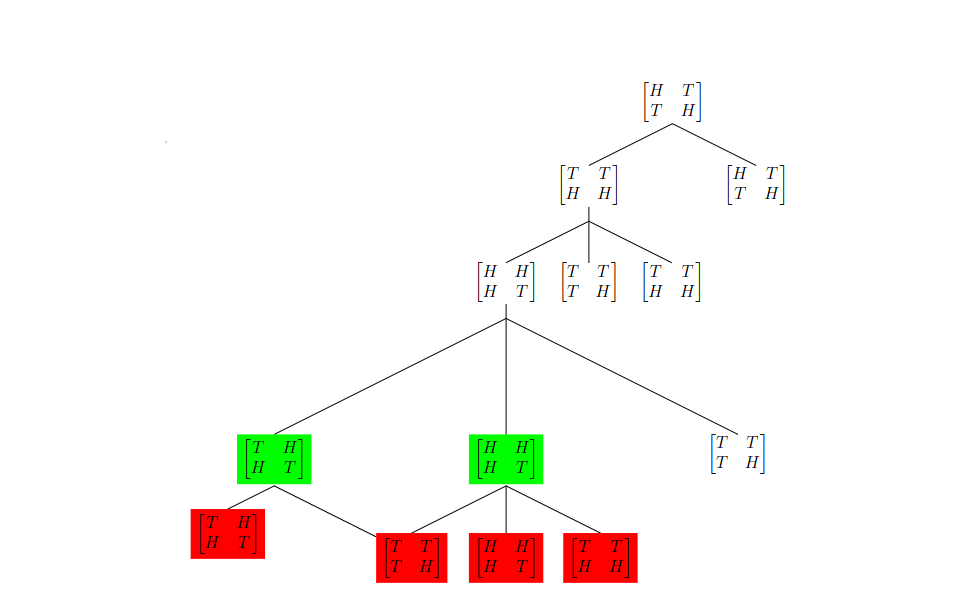
\includegraphics[scale=0.5]{treelast}


\section{Conclusion}

We highlight moves the same colour if they use the same move to move upwards in the tree. Here we notice the red group of states which contains all four non-winning/starting states after one move reduces to a green group of two non-winning states, after that it reduces to one state from there on until the winning state. The closest instance from the root where all four non-winning/starting states use the same method to move to a smaller subset of non-winning states is the group highlighted as red and since this is four moves away {$\begin{bmatrix} H & T \\ T & H \end{bmatrix}$} which itself is one move away from winning hence the best solution must use five moves. 





\end{document}